\documentclass[11pt]{article}
\usepackage{listings}
\usepackage{xcolor}
\usepackage{multirow}
\usepackage{multicol}
\usepackage{xparse}
\usepackage{amsmath}
\usepackage[BoldFont]{xeCJK}
\usepackage[most]{tcolorbox}
\usepackage[T1]{fontenc}

\usepackage{lmodern}

\graphicspath{ {./image/} }
\renewcommand\thesection{Question \ \arabic{section}}
\renewcommand\thesubsection{\arabic{section}-(\alph{subsection})}
\usepackage{hyperref}
\hypersetup{
    colorlinks=true,
    linkcolor=blue,
    filecolor=magenta,      
    urlcolor=cyan,
    pdftitle={習題7 },
    pdfpagemode=FullScreen,
}
\usepackage[a4paper, margin={3cm}]{geometry}
\linespread{1.15}
\lstset{language=C,keywordstyle={\bfseries \color{blue}}}
	

\title{習題7 \\\Large 總體經濟學原理與實習}
\author{B10703033\ 財金一\ 邱奕璉
\\ B10703103\ 財金一\ 許羽婷
\\ B10705007\ 資管一\ 劉冠甫
\\ B10705047\ 資管一\ 邱秉辰}
\date{April 29, 2022}

\setlength{\parindent}{0em}
\setlength{\parskip}{0.5em}

\setCJKmainfont{GenRyuMin TW}
\begin{document}



\maketitle

\section{}
\subsection{}
委內瑞拉，折合新台幣 233.8 元
\subsection{}
越南、瑞士和台灣 \\ 
In April it confirmed that \textbf{Vietnam} was one of a trio of trading partners, alongside \textbf{Switzerland} and \textbf{Taiwan}, pursuing “potentially unfair” currency practices, based on three tests of its devising.
\subsection{}
央行買入大量外匯，使得外匯需求增加，使得升值幅度下降，達到阻止升值的效果
\begin{figure}[h]
    \centering
    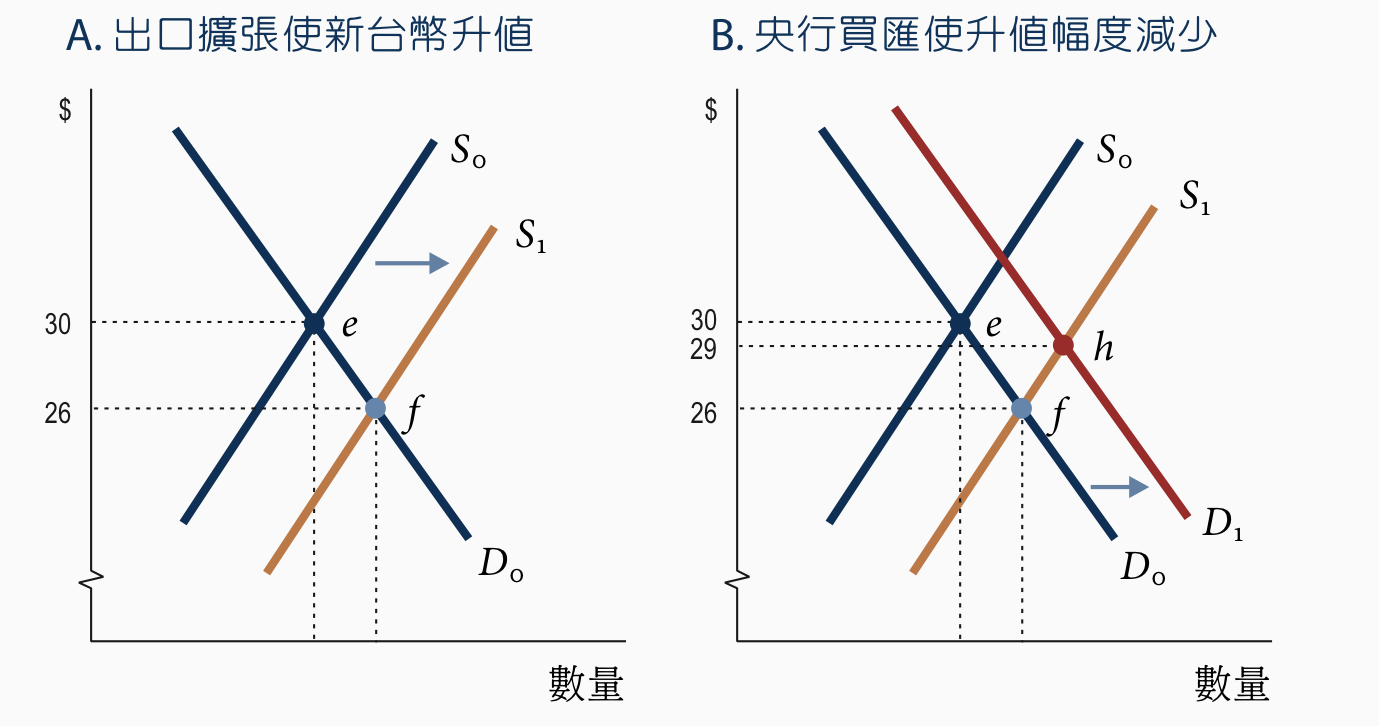
\includegraphics[scale = 0.2]{1c.png}
\end{figure}

\section{}
\subsection{}
央行盈餘 = 國外資產 $\times$  國內外利差 \\ 
由上式可知，由於國內外利率有所差異，因此造成盈餘。
\subsection{}
台灣央行為了阻止新台幣升值，買入大量外匯，使得 2(a) 式中的國外資產增加。
\subsection{}
台灣央行無法決定國外利率，但若將國內利率壓低，便會使得國內外利差變大，由2(a) 式可知此連帶造成盈餘增加。
\subsection{}
由 2(b) 小題可知，盈餘來自進口商（外匯需求者） \\
由 2(c) 小題可知，盈餘來自存款人（利息所得相對變少）

\section{}
$$
(30-28)x = 11563 \\ x= 5781.5\text{(億美元)} 
$$
\section{}
\subsection{}
\begin{enumerate}
    \item 美國： -\$616.095
    \item 中國： \$248.838
    \item 台灣：\$94.956
    \item 全球總和：\$367.942
\end{enumerate}
(單位：十億美元)
\subsection{}
最主要的原因是因為服務業的出入口計算難以衡量，出口者很好匯報自己的出口量，但進口者可能是很多很零星的消費者，這些金額微小的服務進口可能沒有被記入統計。此外，由於貨物延誤以及企業為了減稅所浮報或低報的進出口額也是原因之一。 \\
An IMF study in 2009, by Marco Terrones and Thomas Helbling, concluded that the biggest cause of the switch from a global current-account deficit to a surplus was mismeasurement of services.
\subsection{}
地球對火星的出口大於進口 $\implies$ 地球經常帳總和 $>$ 0
\end{document}



